\section{Construcción del índice: segunda parte}\label{sec:indice2}

Se continuará utilizando el ejemplo.

\subsection{Merge-Based Inversion}

Es inevitable citar a \citet[p. ~14]{Zobel06invertedfiles} (\citeyear{Zobel06invertedfiles}) y \citet[p.~238]{WittenMoffatBell99} (\citeyear{WittenMoffatBell99}), en donde encontramos

Merge-based index construction is practical for collections of all sizes. In particular,
it scales well and operates effectively in as little as 100MB of memory. In addition, disk
space overheads can be restricted to a small fraction of the final index; only one parsing
pass is required over the data; and the method extends naturally to phrase indexing.
Finally, the compression techniques described in Section 8 can further reduce the cost
of index construction by reducing the number of runs required.


%\begin{figure}[!h]
%\centering
%    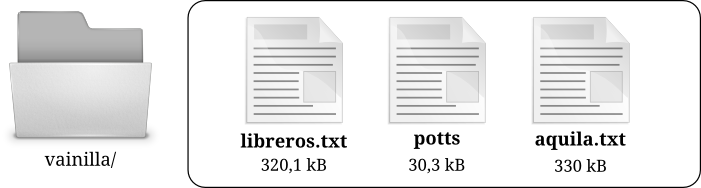
\includegraphics[scale=0.9]{./Images/vainillaDir.png}
%\caption{Ejemplo de directorio de trabajo}
%\label{fig:directorioTrabajo}
%\end{figure}


